% Options for packages loaded elsewhere
\PassOptionsToPackage{unicode}{hyperref}
\PassOptionsToPackage{hyphens}{url}
\PassOptionsToPackage{dvipsnames,svgnames,x11names}{xcolor}
%
\documentclass[
  11pt,
]{ieee}

\usepackage{amsmath,amssymb}
\usepackage{setspace}
\usepackage{iftex}
\ifPDFTeX
  \usepackage[T1]{fontenc}
  \usepackage[utf8]{inputenc}
  \usepackage{textcomp} % provide euro and other symbols
\else % if luatex or xetex
  \usepackage{unicode-math}
  \defaultfontfeatures{Scale=MatchLowercase}
  \defaultfontfeatures[\rmfamily]{Ligatures=TeX,Scale=1}
\fi
\usepackage{lmodern}
\ifPDFTeX\else  
    % xetex/luatex font selection
\fi
%% Support for zero-width non-joiner characters.
\makeatletter
\def\zerowidthnonjoiner{%
  % Prevent ligatures and adjust kerning, but still support hyphenating.
  \texorpdfstring{%
    \TextOrMath{\nobreak\discretionary{-}{}{\kern.03em}%
      \ifvmode\else\nobreak\hskip\z@skip\fi}{}%
  }{}%
}
\makeatother
\ifPDFTeX
  \DeclareUnicodeCharacter{200C}{\zerowidthnonjoiner}
\else
  \catcode`^^^^200c=\active
  \protected\def ^^^^200c{\zerowidthnonjoiner}
\fi
%% End of ZWNJ support
% Use upquote if available, for straight quotes in verbatim environments
\IfFileExists{upquote.sty}{\usepackage{upquote}}{}
\IfFileExists{microtype.sty}{% use microtype if available
  \usepackage[]{microtype}
  \UseMicrotypeSet[protrusion]{basicmath} % disable protrusion for tt fonts
}{}
\makeatletter
\@ifundefined{KOMAClassName}{% if non-KOMA class
  \IfFileExists{parskip.sty}{%
    \usepackage{parskip}
  }{% else
    \setlength{\parindent}{0pt}
    \setlength{\parskip}{6pt plus 2pt minus 1pt}}
}{% if KOMA class
  \KOMAoptions{parskip=half}}
\makeatother
\usepackage{xcolor}
\usepackage[margin=1in]{geometry}
\setlength{\emergencystretch}{3em} % prevent overfull lines
\setcounter{secnumdepth}{-\maxdimen} % remove section numbering
% Make \paragraph and \subparagraph free-standing
\makeatletter
\ifx\paragraph\undefined\else
  \let\oldparagraph\paragraph
  \renewcommand{\paragraph}{
    \@ifstar
      \xxxParagraphStar
      \xxxParagraphNoStar
  }
  \newcommand{\xxxParagraphStar}[1]{\oldparagraph*{#1}\mbox{}}
  \newcommand{\xxxParagraphNoStar}[1]{\oldparagraph{#1}\mbox{}}
\fi
\ifx\subparagraph\undefined\else
  \let\oldsubparagraph\subparagraph
  \renewcommand{\subparagraph}{
    \@ifstar
      \xxxSubParagraphStar
      \xxxSubParagraphNoStar
  }
  \newcommand{\xxxSubParagraphStar}[1]{\oldsubparagraph*{#1}\mbox{}}
  \newcommand{\xxxSubParagraphNoStar}[1]{\oldsubparagraph{#1}\mbox{}}
\fi
\makeatother


\providecommand{\tightlist}{%
  \setlength{\itemsep}{0pt}\setlength{\parskip}{0pt}}\usepackage{longtable,booktabs,array}
\usepackage{calc} % for calculating minipage widths
% Correct order of tables after \paragraph or \subparagraph
\usepackage{etoolbox}
\makeatletter
\patchcmd\longtable{\par}{\if@noskipsec\mbox{}\fi\par}{}{}
\makeatother
% Allow footnotes in longtable head/foot
\IfFileExists{footnotehyper.sty}{\usepackage{footnotehyper}}{\usepackage{footnote}}
\makesavenoteenv{longtable}
\usepackage{graphicx}
\makeatletter
\def\maxwidth{\ifdim\Gin@nat@width>\linewidth\linewidth\else\Gin@nat@width\fi}
\def\maxheight{\ifdim\Gin@nat@height>\textheight\textheight\else\Gin@nat@height\fi}
\makeatother
% Scale images if necessary, so that they will not overflow the page
% margins by default, and it is still possible to overwrite the defaults
% using explicit options in \includegraphics[width, height, ...]{}
\setkeys{Gin}{width=\maxwidth,height=\maxheight,keepaspectratio}
% Set default figure placement to htbp
\makeatletter
\def\fps@figure{htbp}
\makeatother

\usepackage{booktabs}
\usepackage{longtable}
\usepackage{array}
\usepackage{multirow}
\usepackage{wrapfig}
\usepackage{float}
\usepackage{colortbl}
\usepackage{pdflscape}
\usepackage{tabu}
\usepackage{threeparttable}
\usepackage{threeparttablex}
\usepackage[normalem]{ulem}
\usepackage{makecell}
\usepackage{xcolor}
\makeatletter
\@ifpackageloaded{caption}{}{\usepackage{caption}}
\AtBeginDocument{%
\ifdefined\contentsname
  \renewcommand*\contentsname{Table of contents}
\else
  \newcommand\contentsname{Table of contents}
\fi
\ifdefined\listfigurename
  \renewcommand*\listfigurename{List of Figures}
\else
  \newcommand\listfigurename{List of Figures}
\fi
\ifdefined\listtablename
  \renewcommand*\listtablename{List of Tables}
\else
  \newcommand\listtablename{List of Tables}
\fi
\ifdefined\figurename
  \renewcommand*\figurename{Figure}
\else
  \newcommand\figurename{Figure}
\fi
\ifdefined\tablename
  \renewcommand*\tablename{Table}
\else
  \newcommand\tablename{Table}
\fi
}
\@ifpackageloaded{float}{}{\usepackage{float}}
\floatstyle{ruled}
\@ifundefined{c@chapter}{\newfloat{codelisting}{h}{lop}}{\newfloat{codelisting}{h}{lop}[chapter]}
\floatname{codelisting}{Listing}
\newcommand*\listoflistings{\listof{codelisting}{List of Listings}}
\makeatother
\makeatletter
\makeatother
\makeatletter
\@ifpackageloaded{caption}{}{\usepackage{caption}}
\@ifpackageloaded{subcaption}{}{\usepackage{subcaption}}
\makeatother

\ifLuaTeX
  \usepackage{selnolig}  % disable illegal ligatures
\fi
\usepackage{bookmark}

\IfFileExists{xurl.sty}{\usepackage{xurl}}{} % add URL line breaks if available
\urlstyle{same} % disable monospaced font for URLs
\hypersetup{
  pdftitle={COMPARING HRV ACROSS DIFFERENT MEDITATION \& BREATHING TECHNIQUES},
  colorlinks=true,
  linkcolor={blue},
  filecolor={Maroon},
  citecolor={Blue},
  urlcolor={Blue},
  pdfcreator={LaTeX via pandoc}}


\title{COMPARING HRV ACROSS DIFFERENT MEDITATION \& BREATHING
TECHNIQUES}
\author{}
\date{}

\begin{document}
\maketitle


\setstretch{1.15}
\vspace{1cm}

\begin{center}
\large \textbf{Author:}\\[0.25em]
\textbf{Johan Kevin Agatare}\\
\textbf{Patel Maitri Narendrakumar}\\
\textbf{Patel Badal Kiritbhai}
\end{center}

\vspace{0.8cm}

\begin{abstract}

This project compared time-domain heart rate variability (HRV)  metrics—Mean heart rate (Mean-HR), Standard Deviation of NN intervals (SDNN), and Root Mean Square of Successive Differences (RMSSD); across various physiological states—sleep, different meditations, and breathing techniques. 

The data was obtained from the PhysioNet database and was processed to extract heart rate and R-R interval data. Statistical analyses were conducted to explore and identify any differences between physiological states and to enhance understanding of the data. 

Most t-test results revealed no statistically significant differences, but the ANOVA tests revealed significant differences for the metrics of all groups tested. 

Afterward, machine learning models were trained using computed time-domain HRV metrics, which served as input features. Of the machine learning models tested, Logistic regression and SVM achieved the highest classification accuracy of 0.67. 

This project further demonstrated that HRV metrics can be used to distinguish between different physiological states and offered insight for future research.

\end{abstract}
\renewcommand{\IEEEkeywordsname}{Keywords}
\begin{IEEEkeywords}
\scriptsize 
Heart Rate Variability (HRV), time-domain metrics, states, statistical analysis, machine learning models, evaluation metrics, hyperparameter tuning, feature importance, autonomic nervous system, parasympathetic activity, preprocessing, RR intervals, visualization, Python, R, PhysioNet dataset
\end{IEEEkeywords}

\section{I. INTRODUCTION}\label{i.-introduction}

\subsection{Background and
Significance}\label{background-and-significance}

\vspace{0.8em}

The autonomic nervous system balance and response capabilities are
evaluated through Heart Rate Variability (HRV) {[}10{]}, which serves as
a basic biological measurement method {[}11,12{]}. The measure
demonstrates different heartbeat timing patterns, which research teams
associate with emotional management, stress systems, and heart wellness.
Science utilizes HRV more often to observe mindfulness effects as well
as relaxation methods and mental wellness studies {[}1{]}.

People use meditation along with structured breathing techniques as
well-known, non-invasive tools to enhance HRV values. In a sense,
enhancing HRV values is a practice whereby human bodies achieve
emotional equilibrium through these practices that allow both
parasympathetic activation and sympathetic reduction, thus minimizing
stress-related physiological responses. Research about meditative
approaches and their effects on HRV shows insufficient study despite
their common use, so scientists still need to figure out which method
leads to the best results in cardiovascular and nervous.

\subsection{Literature Survey}\label{literature-survey}

\vspace{0.8em}

Current research shows that stress exists as a statistically important
factor related to HRV outcomes. Research by Kim et al.~{[}2{]}, through
meta-analysis demonstrated that stress reduction interventions enhance
HRV measurements because stress affects the autonomic nervous system's
psychological regulation functions. Scientific research has evaluated
the impact that both structured respiration methods and mindful
breathing exercises have on oneself. The study conducted by Natarajan
{[}3{]} revealed that HRV increased with breathing-focused meditation,
which caused an improvement in vagal activity. Short, structured
breathing exercises, according to Balban et al.~{[}4{]}, decreased
stress levels and generated better emotional states in subjects.

Studies about meditation primarily study individual approaches or
analyze meditation relative to minimal restful states. The research
field comprise extensive quantitative comparison of meditative and
breathing techniques when assessing their impact on HRV through
statistical evaluation.

Still, current research does not offer proper implementation of machine
learning techniques to analyze HRV data although such methods could
enable the development of individualized stress management tools.

\subsection{Research Objectives and
Contributions}\label{research-objectives-and-contributions}

\vspace{0.8em}

This project aimed to address the detected research gaps by conducting a
comparative analysis using four different states: \textbf{Meditation
(both before and after), Fixed-rate breathing, and Sleep}.

Specifically, the research :

\begin{itemize}
\item
  Evaluated Time-domain-HRV metrics{[}13,14,15{]}---Mean heart rate,
  SDNN and RMSSD, for each state.
\item
  Analyzed HRV changes by applying ANOVA and t-tests to conduct
  statistical comparisons between the techniques.
\item
  Established if the HRV changes resulting from meditation practices,
  controlled breathing or sleep produced patterns that can be
  differentiated from one another.
\item
  Built machine learning models, such as KNN or Random Forest, to
  classify different physiological states through the analysis of HRV
  time domain features(metrics).
\end{itemize}

This research used predictive models and statistical analysis to
generate two key scientific benefits: a better empirical understanding
of meditation impacts on physiology and the ability to develop systems
that identify relaxation methods using HRV data patterns.

Recent studies showed that heart rate signals during meditation were
inherently non-linear and exhibit fractal and multifractal
characteristics, requiring more sophisticated analysis methods than
conventional time-domain or spectral analysis {[}5,6{]}.

Nasrolahzadeh et al.~{[}5{]}, and Bhaduri and Ghosh {[}6{]} demonstrated
that techniques like \textbf{Visibility Graphs} and \textbf{MF-DFA} can
detect hidden changes in HRV structure during meditation but did not
explore statistical comparisons across techniques or simpler predictive
models.

Looking at studies that used the same dataset and have integrated
machine learning approaches such as \textbf{LSTM} {[}7{]} or others,
with different datasets that used machine learning techniques such as
\textbf{KNN, SVM, K-means clustering} and \textbf{SVC}{[}8,9{]} , this
project expands upon previous works by comparing the HRV effects of
multiple meditation and breathing techniques using interpretable
features and classification methods suitable for real-world
applications.

\section{II. METHODS}\label{ii.-methods}

\subsection{Data description}\label{data-description}

\vspace{0.8em}

This project utilized the ``\emph{Heart Rate Oscillations during
Meditation}'' dataset from PhysioNet{[}6{]}. This dataset contained
heart rate time-series data from five groups:

\begin{itemize}
\item
  \textbf{Chi meditation group} (C1--C8): This group had HRV recordings
  of participants' Pre-meditation and Meditation data (around one hour
  each).
\item
  \textbf{Kundalini Yoga meditation group} (Y1--Y4): which had HRV
  recordings of Pre-meditation and Meditation of participants HRV data
  (17--47 minutes each).
\item
  \textbf{Spontaneous breathing group}(normal group) (N1--N11): This
  group recorded participants' HRVs while sleeping (about 6 hours each).
\item
  \textbf{Metronomic breathing group} (M1--M14): This group had HRV
  recordings while participants were breathing at a fixed rate (0.25 Hz)
  for 10 minutes in a supine position.
\item
  \textbf{Ironman group} (I1-I9): This group had HRV recordings of Elite
  athletes while they were sleeping hours before the Ironman Triathlon
\end{itemize}

Each dataset consisted of time in seconds and instantaneous heart
rate---both normal heart rate in beats per minute and R-R interval
recordings.

\subsection{Method description}\label{method-description}

\vspace{0.8em}

The following time-domain-HRV metrics{[}13,14,15{]} were used:

\begin{itemize}
\item
  \textbf{Mean Heart Rate (Mean-HR)} -- which measures the overall
  cardiovascular response/activity and is easily computed.
\item
  \textbf{Standard Deviation of NN intervals (SDNN)} -- which measures
  overall changes in R-R intervals {[}17{]} and needs to be computed.
\item
  \textbf{Root Mean Square of Successive Differences (RMSSD)} -- which
  is an indicator of parasympathetic nervous system activity {[}17{]},
  uses R-R intervals data and is almost like \textbf{SDNN}, except that
  it is a bit more sensitive to short-term variations in heart rate and
  more directly reflects vagal (parasympathetic) activity{[}18,10{]}.
\end{itemize}

\subsection{Analysis Steps}\label{analysis-steps}

\vspace{0.8em}

\begin{enumerate}
\def\labelenumi{\arabic{enumi}.}
\item
  First HRV metrics(both normal heart rate and R-R intervals) were
  extracted for each group(\textbf{Chi, Yoga, Normal sleep, Ironman
  group, Metronomic breathing}). Later, normal \textbf{heart rate and
  R-R interval} data for each group were merged into one dataset for
  heart rate data(for each group) and one dataset for R-R intervals(for
  each group). Resulting in a total of \textbf{10} datasets( \textbf{5}
  heart rate datasets and 5 R-R intervals dataset). For detailed summary
  of how the data was processed, and transformed refer to:
  \emph{Chi\_C1\_Data\_Preprocessing\_Summary.docx,
  Chi\_C1\_RR\_Interval\_Summary.docx, and
  Chi\_Final\_Merged\_Datasets\_Summary.docx}.
\item
  Second, afterward, \textbf{Mean-HR, SDNN, and RMSSD} were computed for
  all groups and later on, merged together into one data set containing
  all the HRV metrics(Mean-HR, SDNN, and RMSSD) for all
  groups(``\emph{o\_1\_all\_hrv\_rr\_metric\_combined}'').\\
\item
  For easy comparison, all groups that featured common practices were
  grouped together:

  \begin{itemize}
  \item
    \emph{\texttt{Chi\ meditation}} and \emph{\texttt{Yoga\ meditation}}
    were grouped together under \emph{\texttt{Pre-meditation}} and
    \emph{\texttt{Meditationstate(condition)}}.
  \item
    The \emph{\texttt{Spontaneous\ breathing\ group}} and the
    \emph{\texttt{Ironman\ group}} that practiced normal breathing while
    \emph{\texttt{sleeping}} were grouped under the
    \emph{\texttt{sleep}} state.
  \item
    The \emph{\texttt{Metronomic\ breathing\ group}} was under
    \emph{\texttt{Fixed-rate\ breathing}} state.
  \end{itemize}
\item
  HRV data of \textbf{Chi} group and \textbf{Yoga} group were evaluated
  using \textbf{Shapiro-Wilk tests} which assess data
  \textbf{normality}. After that the changes in Pre-meditation
  vs.~Meditation were evaluated using a \textbf{`paired t-test'}.
\item
  HRV changes in \textbf{Meditation} vs.~\textbf{sleep}
  vs.~\textbf{fixed-rate breathing} were evaluated using
  `\textbf{one-way ANOVA}'.
\item
  Multiple machine learning models were trained to
  classify(differentiate) between states based on HRV features(metrics).
  The chosen models were \textbf{\emph{K-Nearest Neighbors (KNN), Random
  Forest, Logistic regression, Support vector machine(SVM), and Gradient
  boosting classifier}}
\end{enumerate}

Finally, the evaluation metrics used were \textbf{Accuracy},
\textbf{Confusion Matrix}, \textbf{F1-score} and \textbf{GridSearchCV}
was used for \textbf{hyperparameters tuning}.

\subsubsection{Tools}\label{tools}

\vspace{0.8em}

The programming Language used was \textbf{Python} alongside the
following libraries:
\texttt{Pandas,\ NumPy,\ SciPy\ (Statistical\ Analysis),\ Matplotlib\ \&\ Seaborn\ (Visualization),\ Scikit-learn\ (Machine\ Learning),\ WFDB\ (PhysioNet\ data\ processing)}.
For development \textbf{Jupyter Lab} was used and for visualization and
rendering \textbf{R studio}.

\section{III. RESULTS}\label{iii.-results}

This section presents the outcomes of statistical analysis and machine
learning models. Statistical analysis was conducted in order to assess
HRV differences across states(conditions) and groups using time-domain
metrics. Machine learning classification was performed in order to
classify physiological states based on the same HRV time-domain metrics.
And the following table shows how the final dataset after preprocessing
and transformation(see table I).

\begin{table}[!h]
\centering
\caption{Sample HRV metrics: First 10}
\centering
\resizebox{\ifdim\width>\linewidth\linewidth\else\width\fi}{!}{
\begin{tabular}[t]{lrlrrll}
\toprule
Subject & Mean\_HR & State & SDNN & RMSSD & Group & Label\\
\midrule
C1\_pre & 71.0277 & Pre-Meditation & 0.1193 & 0.1550 & Chi & Pre-Meditation\\
C1\_med & 73.7491 & Meditation & 0.0485 & 0.0187 & Chi & Meditation\\
C2\_pre & 83.9852 & Pre-Meditation & 0.0762 & 0.0674 & Chi & Pre-Meditation\\
C2\_med & 82.3966 & Meditation & 0.0472 & 0.0556 & Chi & Meditation\\
C3\_pre & 84.2524 & Pre-Meditation & 0.0654 & 0.0263 & Chi & Pre-Meditation\\
\addlinespace
C3\_med & 74.7653 & Meditation & 0.0407 & 0.0224 & Chi & Meditation\\
C4\_pre & 84.6186 & Pre-Meditation & 0.0690 & 0.0188 & Chi & Pre-Meditation\\
C4\_med & 75.4436 & Meditation & 0.0515 & 0.0198 & Chi & Meditation\\
C5\_pre & 77.4535 & Pre-Meditation & 0.0336 & 0.0138 & Chi & Pre-Meditation\\
C5\_med & 67.8328 & Meditation & 0.0310 & 0.0152 & Chi & Meditation\\
\bottomrule
\end{tabular}}
\end{table}

\subsection{Normality results: Chi and Yoga
group.}\label{normality-results-chi-and-yoga-group.}

\vspace{0.8em}

\begin{table}[!h]
\centering
\caption{Normality results for the Chi group}
\centering
\resizebox{\ifdim\width>\linewidth\linewidth\else\width\fi}{!}{
\begin{tabular}[t]{llrr}
\toprule
Metric & Group\_State & W-Statistic & p-Value\\
\midrule
RMSSD & Chi\_pre & 0.7362 & 0.0057\\
RMSSD & Chi\_med & 0.8149 & 0.0413\\
SDNN & Chi\_pre & 0.9098 & 0.3524\\
SDNN & Chi\_med & 0.9547 & 0.7586\\
Mean\_HR & Chi\_pre & 0.8863 & 0.2162\\
\addlinespace
Mean\_HR & Chi\_med & 0.8596 & 0.1190\\
\bottomrule
\end{tabular}}
\end{table}

\textbf{Shapiro-Wilk} tests were conducted to assess data normality
within the \textbf{Chi} and \textbf{Yoga} groups. The results revealed
that for the \textbf{Chi} group, \textbf{RMSSD} was not normally
distributed in either \textbf{pre-meditation} or \textbf{meditation}
states(\textbf{p = 0.0057 and p = 0.0413}). \textbf{SDNN} and
\textbf{Mean-HR} followed a normal distribution for both
states(pre-meditation or meditation). For the \textbf{Yoga} group, all
HRV metrics for both states(pre-meditation or meditation) passed the
normality check with a \textbf{p-value} \textgreater{} \textbf{0.05}(see
table II, III).

\begin{table}[!h]
\centering
\caption{Normality results for the Yoga group}
\centering
\resizebox{\ifdim\width>\linewidth\linewidth\else\width\fi}{!}{
\begin{tabular}[t]{llrr}
\toprule
Metric & Group\_state & W-Statistic & p-Value\\
\midrule
RMSSD & Yoga\_pre & 0.7934 & 0.0989\\
RMSSD & Yoga\_med & 0.9118 & 0.4243\\
SDNN & Yoga\_pre & 0.8753 & 0.3106\\
SDNN & Yoga\_med & 0.9376 & 0.5179\\
Mean\_HR & Yoga\_pre & 0.8184 & 0.1593\\
\addlinespace
Mean\_HR & Yoga\_med & 0.9884 & 0.7942\\
\bottomrule
\end{tabular}}
\end{table}

\subsection{Paired t-test results: Chi and Yoga meditation
groups.}\label{paired-t-test-results-chi-and-yoga-meditation-groups.}

\vspace{0.8em}

\textbf{Paired t-tests} were performed to compare HRV metrics before and
during Meditation for the \textbf{Chi and Yoga} groups. For the
\textbf{Chi} group, none of the metrics showed a \textbf{statistically
significant change}. On the other hand, the \textbf{Yoga} group showed a
statistically significant change in \textbf{Mean-HR, but RMSDD} and
\textbf{SDNN} did not show any(see table IV).

\begin{table}[!h]
\centering
\caption{T-Test results for Chi and Yoga}
\centering
\resizebox{\ifdim\width>\linewidth\linewidth\else\width\fi}{!}{
\begin{tabular}[t]{lrrrr}
\toprule
Metric & Chi\_t & Chi\_p & Yoga\_t & Yoga\_p\\
\midrule
RMSSD & 1.012 & 0.3386 & 0.376 & 0.7282\\
Mean\_HR & 0.826 & 0.4264 & -3.641 & 0.0250\\
SDNN & 2.014 & 0.0795 & 0.021 & 0.9847\\
\bottomrule
\end{tabular}}
\end{table}

\subsection{ANOVA results.}\label{anova-results.}

\vspace{0.8em}

A \textbf{one-way ANOVA} was performed to determine if there were any
significant differences in HRV metrics across the experimental groups.
The results of the ANOVA testing showed that all HRV metrics showed a
significant difference(\textbf{p\textless0.05})(see table V).

\begin{table}[!h]
\centering
\caption{ANOVA results}
\centering
\resizebox{\ifdim\width>\linewidth\linewidth\else\width\fi}{!}{
\begin{tabular}[t]{lrr}
\toprule
Metric & f-Statistic & p-Value\\
\midrule
RMSSD & 4.725 & 0.0141\\
SDNN & 13.274 & 0.0000\\
Mean\_HR & 19.379 & 0.0000\\
\bottomrule
\end{tabular}}
\end{table}

\subsection{Model performance.}\label{model-performance.}

\vspace{0.8em}

The following is a summary of the performances of the different machine
learning models used(see table VI). \textbf{Logistic regression} and
\textbf{Support vector machine}(SVM) had the \textbf{highest accuracy}
and \textbf{F1-score}.

\begin{table}[!h]
\centering
\caption{Machine learning model results}
\centering
\resizebox{\ifdim\width>\linewidth\linewidth\else\width\fi}{!}{
\begin{tabular}[t]{lrr}
\toprule
Model & Accuracy & F1-score\\
\midrule
KNN (Before Tuning) & 0.50 & 0.50\\
KNN (After Tuning) & 0.50 & 0.50\\
Random Forest & 0.58 & 0.59\\
Random Forest (Tuned) & 0.58 & 0.59\\
Logistic Regression & 0.67 & 0.67\\
\addlinespace
Support Vector Machine & 0.67 & 0.68\\
Gradient Boosting & 0.50 & 0.49\\
\bottomrule
\end{tabular}}
\end{table}

\subsection{Line plot for KNN.}\label{line-plot-for-knn.}

\vspace{0.8em}

The following plot showed all the different values of `\textbf{k}'(
\textbf{number of neighbors}) on the \textbf{x-axis} ranging from 1 to
20, and the \textbf{y-axis} showed the \textbf{accuracy}. The purpose of
this plot was to determine which optimal value of k would yield the best
accuracy rather than selecting an arbitrary value that might
underperform(see figure 1).

\begin{figure}

{\centering 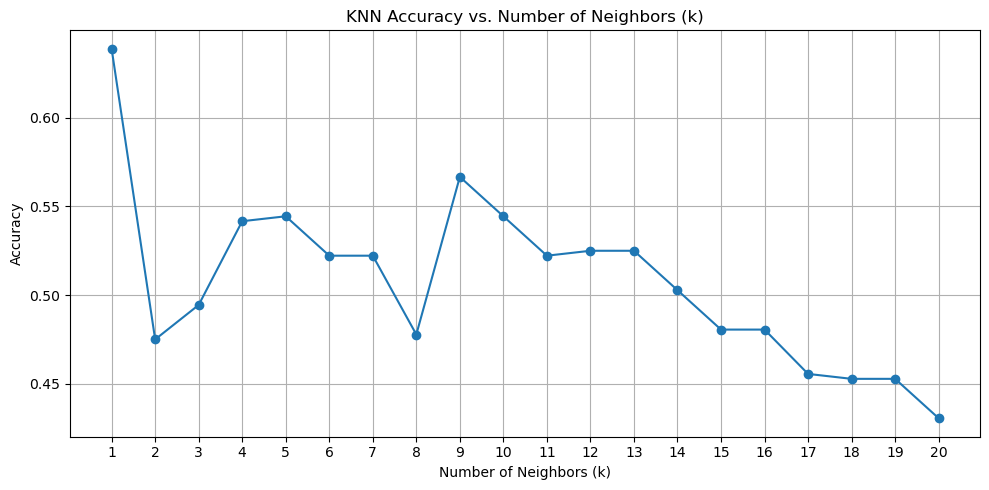
\includegraphics{picture_use_ml/1_Accuracy_for_KNN.png}

}

\caption{Accuracy vs Number of Neighbors}

\end{figure}%

\subsection{Confusion matrix for KNN.}\label{confusion-matrix-for-knn.}

\vspace{0.8em}

This confusion matrix displays the actual versus predicted class for the
\textbf{KNN} model. Diagonal values indicate \textbf{accurate
predictions}, and non-diagonal values indicate
\textbf{misclassifications}. \textbf{Fixed-rate breathing} and
\textbf{Sleeping} showed better classification \textbf{accuracy}, unlike
Pre-\textbf{meditation} and \textbf{Meditation}(see figure 2).

\begin{figure}

{\centering 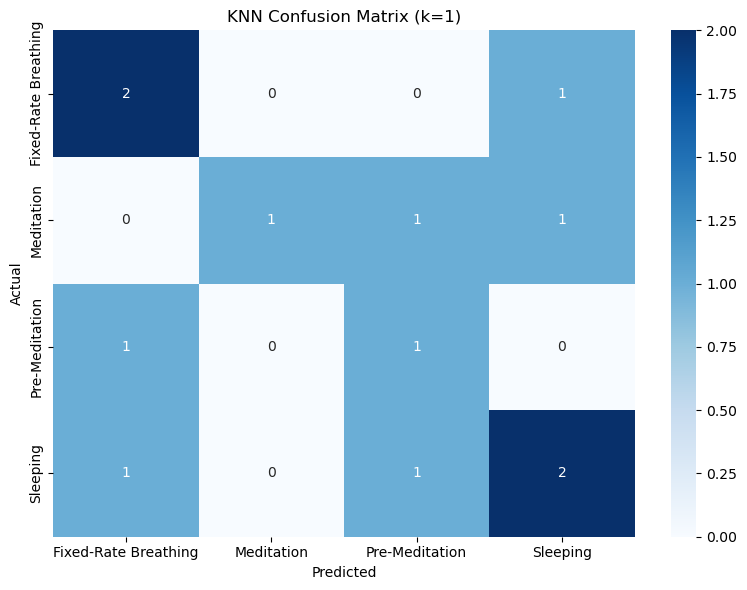
\includegraphics{picture_use_ml/2_Confusion_Matrix_for_KNN.png}

}

\caption{KNN confusion matrix}

\end{figure}%

And the same pattern was observed after \textbf{hyperparameter
tunning}(see figure 3), indicating that the tunning did not have much of
an effect.

\begin{figure}

{\centering 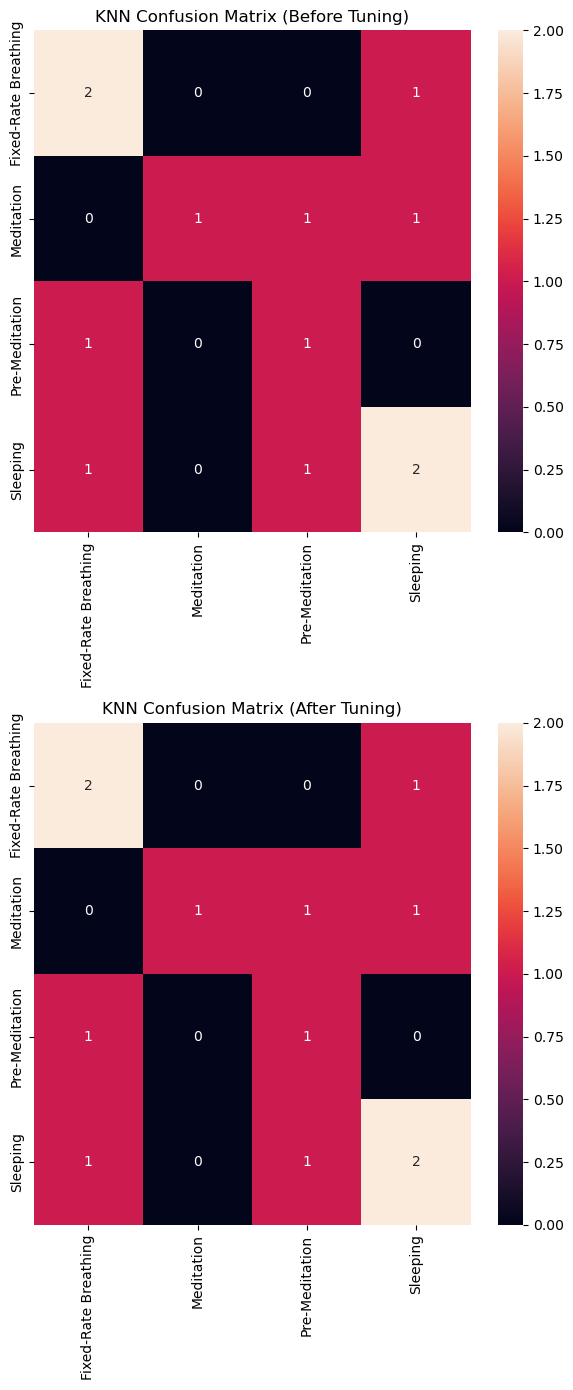
\includegraphics{picture_use_ml/3_KNN Confusion Matrix_Before vs After Tuning.png}

}

\caption{KNN confusion matrix: with tunning}

\end{figure}%

\subsection{Boxplots of HRV metrics by
condition.}\label{boxplots-of-hrv-metrics-by-condition.}

\vspace{0.8em}

The computed \textbf{boxplots} showed the distributions of \textbf{SDNN,
RMSDD, and Mean-HR} across all conditions. These visualizations allow us
to observe whether the selected features display any variabilities that
distinguish them from one another. For instance, \textbf{Mean-HR} was
the highest during \textbf{Meditation}, and \textbf{Fixed-rate
breathing} had low \textbf{SDNN} and \textbf{RMSSD}(see figure 4, 5, 6).

\begin{figure}

{\centering 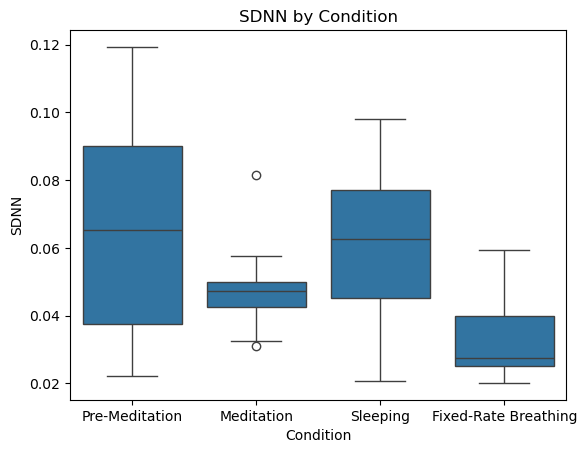
\includegraphics{picture_use_ml/4_Boxplots of HRV Metrics by Condition_SDNN.png}

}

\caption{Boxplot for SDNN distribution}

\end{figure}%%
\begin{figure}

{\centering 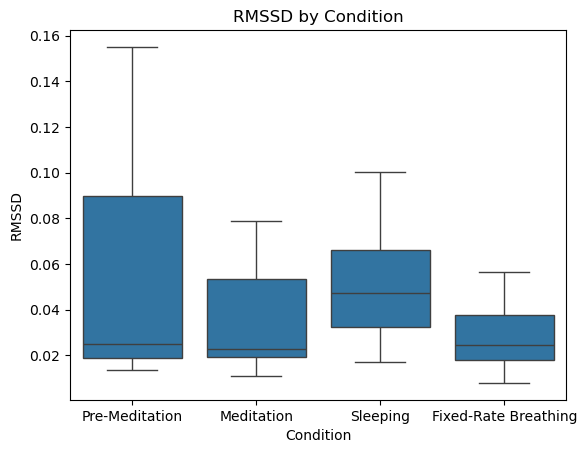
\includegraphics{picture_use_ml/5_Boxplots of HRV Metrics by Condition_RMSDD.png}

}

\caption{Boxplot for RMSDD}

\end{figure}%%
\begin{figure}

{\centering 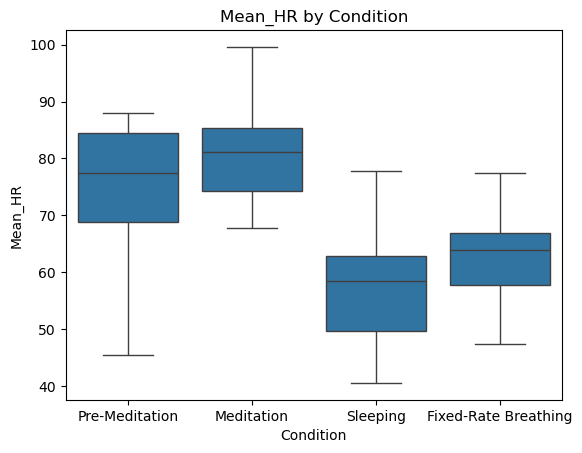
\includegraphics{picture_use_ml/6_Boxplots of HRV Metrics by Condition_Mean_Hr.png}

}

\caption{Boxplot for Mean-HR distribution}

\end{figure}%

\subsection{PCA projection of HRV
features.}\label{pca-projection-of-hrv-features.}

\vspace{0.8em}

\textbf{PCA projection} helped visualize how well the different
conditions clustered compared to one another. While there was some
overlapping, there was a relatively noticeable separation between
Sleeping and fixed-rate breathing(see figure 7).

\begin{figure}

{\centering 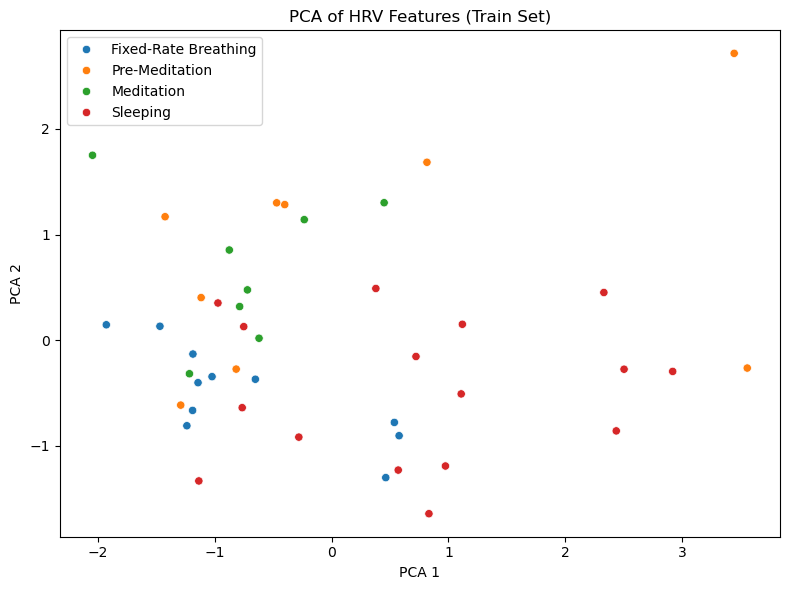
\includegraphics{picture_use_ml/7_PCA Projection of HRV Features.png}

}

\caption{PCA projection}

\end{figure}%

\subsection{Confusion matrix: Random
forest.}\label{confusion-matrix-random-forest.}

\vspace{0.8em}

The confusion matrix for \textbf{random forest} showed better
classification performance compared to \textbf{KNN}. Still, some
misclassifications also occurred, further confirming the possibility of
overlap in the HRV features between certain physiological states(see
figure 8).

\begin{figure}

{\centering 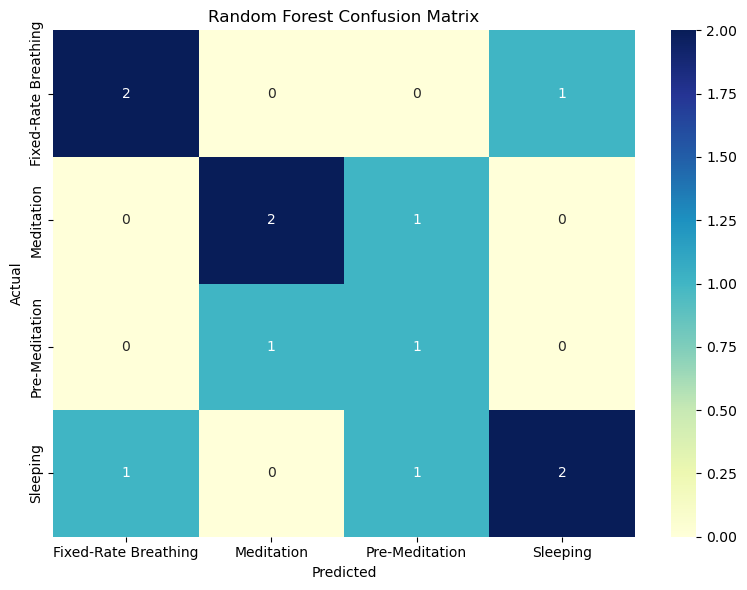
\includegraphics{picture_use_ml/8_Confusion Matrix_ Random Forest.png}

}

\caption{Random forest confusion matrix}

\end{figure}%

In addition, the following confusion matrix(see figure 9) gives a
comparison, showing the improvements of \textbf{Random forest over KNN}.
And allows us to see that Random forest appears to be able to classify
\textbf{Meditation} and \textbf{Pre-meditation} better than \textbf{KNN}
does.

\begin{figure}

{\centering 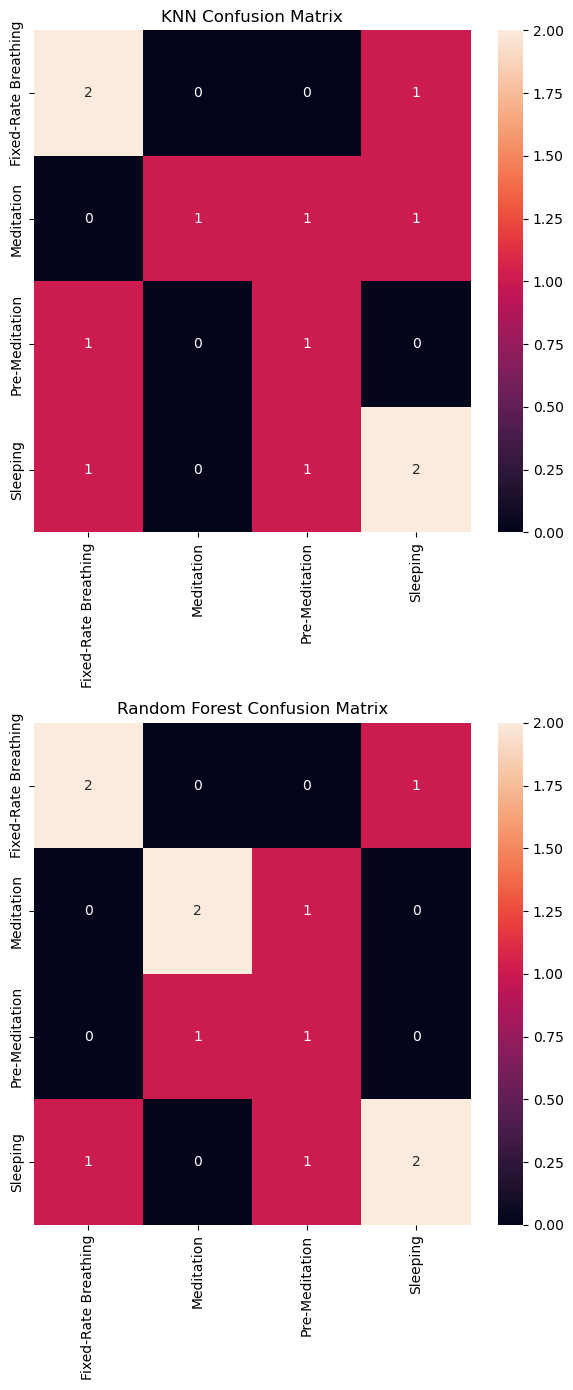
\includegraphics{picture_use_ml/10_Confusion Matrices_KNN vs Random Forest.png}

}

\caption{KNN vs RF confusion matrix}

\end{figure}%

\subsection{Feature importance: Random
forest.}\label{feature-importance-random-forest.}

\vspace{0.8em}

This bar chart showed the rankings of the different features and helped
in determining which ones were the most important---i.e., had the most
predictive power. \textbf{Mean-HR} and \textbf{SDNN} were the most
important, followed by \textbf{RMSSD}(see figure 10).

\begin{figure}

{\centering 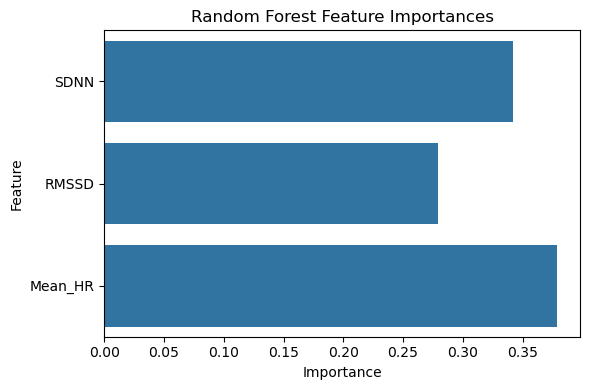
\includegraphics{picture_use_ml/9_Feature Importance_Random Forest.png}

}

\caption{Feature importance}

\end{figure}%

\subsection{Confusion matrices: Logistic regression, SVM, Gradient
boosting.}\label{confusion-matrices-logistic-regression-svm-gradient-boosting.}

\vspace{0.8em}

These matrices give a comparison of the performance of three additional
models that were used. \textbf{Logistic regression} and \textbf{SVM}
showed a \textbf{better classification accuracy} and were able to
identify most of the states. On the other hand, \textbf{Gradient
boosting} seemed to have struggled and misclassified multiple states(see
figure 11).

\begin{figure}

{\centering 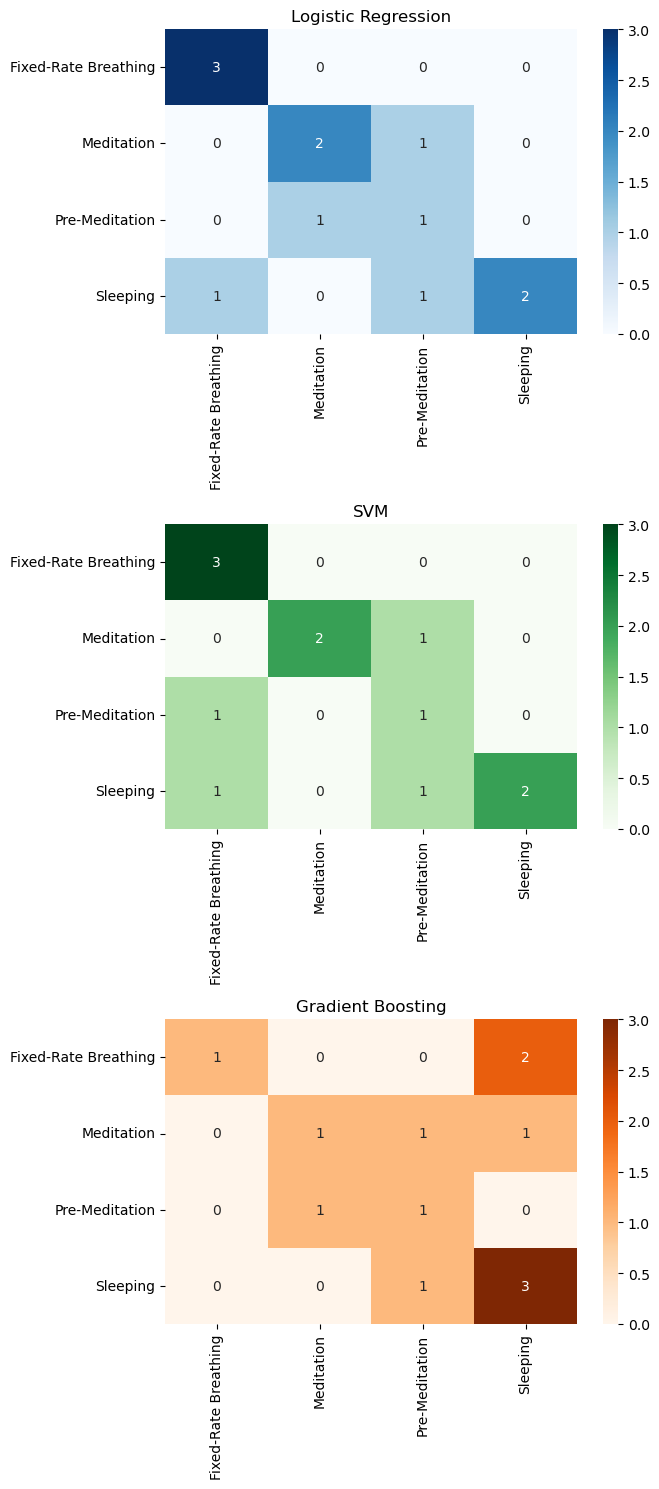
\includegraphics{picture_use_ml/11_Confusion_Matrices_ Logistic_Regressio_SVM_Gradient_Boosting.png}

}

\caption{Confusion matrices}

\end{figure}%

\section{IV. DISCUSSION}\label{iv.-discussion}

The main objective of this project was to evaluate and compare the
effects of different meditation techniques, breathing techniques, and
sleep on \textbf{Heart Rate Variability(}HRV\textbf{)}---a recognized
indicator of autonomic nervous activity, and to determine if a machine
learning model would accurately distinguish between physiological states
computed using time-domain metrics (\textbf{SDNN, RMSSD, Mean-HR}).

The dataset used contained data for five different experimental groups
for which \textbf{Heart rate}( in beats/min) and \textbf{R-R} intervals
were recorded. The groups had different recording times. Some had 10
minutes of recordings, whereas others had up to 4 hours of HR and R-R
recordings.

The findings from both statistical testing and predictive modeling are
discussed below.

\subsection{Normality Test}\label{normality-test}

\vspace{0.8em}

The \textbf{normality test} was conducted to evaluate whether or not the
data was normally distributed and was performed before the paired
t-test. In this case, normality helps assess the data distribution, so
as to have an idea of what to expect. If the \textbf{p-value \textless{}
0.005}, the data is \textbf{not normally} distributed. And, if the
\textbf{p-value \textgreater{} 0.005}, the data is \textbf{normally}
distributed.

The results revealed that \textbf{RMSSD} was not normally distributed in
the \textbf{Chi} group for both conditions(\textbf{pre-meditation and
meditation}). However, \textbf{SDNN and Mean-HR} passed the normality
check.

On the other hand, all HRV metrics for the Yoga group were normally
distributed(\textbf{p \textgreater{} 0.05)}. The statistical testing
proceeded with paired t-test calculations.

Although \textbf{RMSSD} did not meet the normality check, the
\textbf{t-test} was conducted regardless because the goal was to
determine if there were meaningful changes between the pre-meditation
and meditation conditions.

\subsection{T-Test Results}\label{t-test-results}

\vspace{0.8em}

For this project, a \textbf{paired t-test} was conducted for the
\textbf{Chi} and \textbf{Kundalini Yoga} meditation groups. The goal was
to determine if, in fact, the meditation sessions resulted in a
meaningful changes in HRV compared to the pre-meditation baseline.

Establishing such differences would potentially help set expectations
for the subsequent performance of machine learning models tasked with
distinguishing between physiological states. The metrics of choice used
for testing were \textbf{RMSDD, SDNN, and Mean-HR}.

The \textbf{paired t-test} revealed no statistically significant changes
in \textbf{RMSDD, SDNN, or Mean-HR} between \textbf{pre-meditation and
meditation} states in the \textbf{Chi} group.

While \textbf{SDNN} was closer to the significance threshold(\textbf{p =
0.0795}), it was still higher. The lack of significant changes across
all used metrics suggested that \textbf{Chi} meditation may not induce
any HRV changes significant enough to be detected by time-domain
measurements.

On the other hand, the \textbf{Kundalini Yoga} group showed an overall
reduction in \textbf{Mean-HR} during meditation(\textbf{p = 0.0250}),
which was \textbf{statistically significant}. And indicates the
potential calming effect(stress-reduction effect) of meditation on
cardiac function. This supports prior findings that argue that
meditation can activate parasympathetic activity and reduce heart rate.
However, in \textbf{SDNN}(p = 0.9847) or \textbf{RMSSD}(p = 0.7282) for
\textbf{Kundalini Yoga}, no \textbf{statistically significant changes}
were observed, suggesting that, although a reduction in \textbf{Mean-HR}
was observed, the changes were not consistent across all metrics used,
raising questions about the extent to which these effects can be
generalized.

Based on the results of the paired t-test, in most cases there were no
meaningful changes after meditation, suggesting that \textbf{either
better or more sensitive metrics} should be used or that the
physiological effects of meditation might not be easily captured by
\textbf{time-domain} \textbf{metrics}.

\subsection{ANOVA Results}\label{anova-results}

\vspace{0.8em}

A \textbf{One-way ANOVA} test was also performed. Unlike the t-test, the
ANOVA test sought to answer whether the \textbf{HRV metrics}(RMSSD,
SDNN, Mean-HR) differ significantly across multiple physiological states
--\textbf{Sleep, Breathing, or Meditation state}. This analysis would be
helpful, as it could provide insight into the degree of separation that
exists between the different states(conditions).

The results showed that there was a significant difference across all
groups for all three HRV metrics\textbf{(p\textless0.05}).
\textbf{Mean-HR} had the strongest statistical effect(F = 19.379, p
\textless{} 0.0001), followed by \textbf{SDNN} (F = 13.274, p
\textless{} 0.0001), and \textbf{RMSSD} (F = 4.725, p = 0.0141).
\textbf{These findings indicated that HRV patterns differed
significantly between the groups, enough that the difference could be
captured by One-way ANOVA testing.}

The relatively large \textbf{F-values} for \textbf{Mean-HR} and
\textbf{SDNN} suggest substantial \textbf{variation} from one
physiological state to another, indicating their potential usefulness as
features for classification purposes with machine learning models.

At this point, the next step for One-way ANOVA testing will be to
perform a \textbf{post-hoc test} with \textbf{Tukey's HSD}. This is
because when ANOVA returns a result that is significant\textbf{(p
\textless{} 0.05}), it implies the existence of a difference between the
groups, and it is followed up with post hoc tests to discover which
groups differ from one another and how much they differ.

However, in this case, finding out which group differs from one another,
will be useful for classification, which is what the machine learning
will be working on. As such, there is no need to perform the
\textbf{post-hoc} test since the models will act as more or less
\textbf{post-hoc discriminators}. In this case, ANOVA testing confirms
\textbf{feature relevance}, and \textbf{classification models} will
discriminate between the states.

\subsection{Model Performance and
Implications}\label{model-performance-and-implications}

\vspace{0.8em}

For this project, five models were used: \textbf{K-nearest neighbors
(KNN), Random Forest, Logistic Regression, Support Vector Machine (SVM),
and Gradient Boosting Classifier(GBC)}. Of the models assessed,
\textbf{Logistic regression and Support Vector Machine} performed the
best, with an accuracy of \textbf{0.67}( for both ) and an \textbf{F1
score} of \textbf{0.67 and 0.68}, respectively.

These results suggest that even with simple features, it is possible for
the machine learning models to distinguish between \textbf{meditation,
sleep, and breathing states} with moderate accuracy. However, the
effectiveness of linear models like \textbf{Logistic regression} over
complex ones like \textbf{Random forest}, in this context, might shed
light on the underlying structure of the \textbf{HRV} data, which was
found to form distinct cluster when visualized through PCA.

Specifically, the \textbf{PCA} visualization was used to assess whether
the HRV features were distinct from one another. It showed
\textbf{clustering} for \textbf{Sleeping and Fixed-Rate breathing}
groups. And overlaps in the Meditation and Pre-Meditation groups, which
did not come as a surprise as the \textbf{normality test} performed
prior, indicated that the data was not normally distributed, and the
\textbf{t-test} that did not show any significance---\textbf{further
strengthening the notion that there were not enough differences between
the time-domain metrics of these two states}(Meditation and
Pre-Meditation).

In contrast, \textbf{Random forest} and \textbf{KNN} achieved an
accuracy of \textbf{0.58 and 0.50}, respectively---even after tuning,
followed by \textbf{Gradient boosting} at 0.50 as well. \textbf{Random
forest} and \textbf{KNN} achieved an \textbf{F1 score} \textbf{of 0.59
and 0.50}, respectively, followed by \textbf{Gradient boosting} with the
lowest \textbf{F1 score of 0.49}, despite its complexity.

Although \textbf{Random forest} performed better than \textbf{KNN}, it
still underperformed when compared to \textbf{SVM} and \textbf{logistic
regression}. Furthermore, rankings of \textbf{feature importance} from
the \textbf{random forest} model indicated that \textbf{Mean-HR and
SDNN}, probably contributed the most to prediction \textbf{accuracy},
which aligns with existing literature that identified these metrics as
good indicators of physiological state.

The \textbf{low performance of KNN} might be attributed to the limited
number of \textbf{features} and potentially the \textbf{overlapping}
distributions of HRV metrics across classes(HRV metrics), as shown by
the boxplots, which in turn could be responsible for the model's
inability to clearly distinguish between the different
conditions(physiological states).

In this instance, the computed \textbf{boxplot} showed some trends, like
elevated \textbf{Mean-HR} during \textbf{meditation}, but offered
evidence that suggests the metrics used might not be enough for accurate
classification. However, consistent patterns were observed, which helped
justify their inclusion.

The comparison between the selected models further emphasized the
importance of model complexity versus data characteristics. It also
confirmed that though \textbf{time-domain HRV} features can be used for
modeling physiological states, they may require additional features to
improve accuracy.

Furthermore, the confusion matrix also showed that although
\textbf{Random Forest and SVM} could accurately classify
\textbf{Sleeping} and \textbf{Meditation} states,
\textbf{Pre-Meditation} and \textbf{Fixed-rate breathing states} were
more commonly misclassified, especially by \textbf{KNN} and
\textbf{Gradient boosting}. This further suggests that the physiological
states produced HRV patterns that overlapped, making accurate
classification challenging.

\subsection{Why Simpler Models Performed
Better}\label{why-simpler-models-performed-better}

\vspace{0.8em}

As evidenced by the performance table, simple models like
\textbf{logistic regression} performed better than complex ones like
\textbf{Gradient boosting}.

This could be due to the \textbf{small set of features} and a
\textbf{dataset that was not large enough}. In addition, \textbf{feature
importance} from random forest showed that \textbf{Mean-HR and SDNN}
were the most important variables, reinforcing the findings from ANOVA
results. RMSDD, on the other hand, did not show the same degree of
predictive power, although not far behind from the other features.

\section{V. CONCLUSION}\label{v.-conclusion}

All in all, the results of this study demonstrated that \textbf{Heart
rate variability(HRV) metric}---\textbf{SDNN, RMSDD}, and
\textbf{Mean-HR}; can capture useful distinctions between
\textbf{sleeping, meditative, and breathing states}, which can be used
for \textbf{classification and comparison} purposes, thereby supporting
previous literature that used HRV as a useful marker of autonomic
activity. Both statistical testing(\textbf{t-tests, ANOVA}) and machine
learning models highlighted the discriminative power of time domain
metrics--- particularly for \textbf{Mean-HR} and \textbf{SDNN}.

In addition, the good performance of \textbf{SVM} and \textbf{Logistic
regression} suggests that even simple physiological data can be used to
build predictive models, rendering the feasibility of automated
physiological state detection, possible.

Furthermore, these findings confirm that a combination of statistical
analysis and machine learning can enable both understanding and
classification of physiological states using simple heart rate data.

And from a practical standpoint, this opens the door for real-time
applications in wearable devices that could be used for monitoring
sleep, breathing, or meditation.

Future studies could seek to enhance model performance by including
additional features (e.g., \textbf{frequency-domain or non-linear HRV
metrics}), \textbf{increasing sample sizes}, or using \textbf{deep
learning} methods to extract raw RR intervals.

\subsection{Limitations}\label{limitations}

\vspace{0.8em}

Although initially, the data was relatively large, preprocessing and
transformation reduced its size significantly and possibly introduced
class(variable) imbalance, which may have limited its generalizability.

Furthermore, although time-domain metrics(features) have proven useful
and easy to interpret, they may fail to accurately capture and
distinguish the complex and different patterns of autonomic nervous
system activity.

And even though moderate classification accuracy was obtained, the
persistent rate of misclassification suggests that better models or
features should be used.

Lastly, the inclusion of the ``Pre-meditation'' state/condition, could
have potentially increased the misclassification rate since its
physiological features likely overlap with meditative and
resting(sleeping or fixed breathing) states.

\newpage

\section{VI.References}\label{vi.references}

{[}1{]} R. Tiwari et al., ``Analysis of Heart Rate Variability and
Implication of Different Factors on Heart Rate Variability,'' Curr.
Cardiol. Rev., vol.~17, no. 5, Oct.~2021. {[}Online{]}. Available:
\url{https://www.ncbi.nlm.nih.gov/pmc/articles/PMC8950456/}

{[}2{]} H.-G. Kim et al., ``Stress and Heart Rate Variability: A
Meta-Analysis and Review,'' Psychiatry Investig., vol.~15, no. 3,
pp.~235--245, Mar.~2018. {[}Online{]}. Available:
\url{https://www.ncbi.nlm.nih.gov/pmc/articles/PMC5900369/}

{[}3{]} A. Natarajan, ``Heart rate variability during mindful breathing
meditation,'' Front. Physiol., vol.~13, 2023. {[}Online{]}. Available:
\url{https://www.frontiersin.org/articles/10.3389/fphys.2022.1017350/full}

{[}4{]} M. Y. Balban et al., ``Brief structured respiration practices
enhance mood and reduce physiological arousal,'' Cell Rep.~Med., vol.~4,
no. 1, Jan.~2023. {[}Online{]}. Available:
\url{https://www.cell.com/cell-reports-medicine/fulltext/S2666-3791(22)00474-8}

{[}5{]} M. Nasrolahzadeh et al., ``A novel method for distinction heart
rate variability during meditation using LSTM recurrent neural networks
based on visibility graph,'' Biomed. Signal Process. Control, vol.~90,
2024. {[}Online{]}. Available:
\url{https://doi.org/10.1016/j.bspc.2023.105822} {[}6{]} A. Bhaduri and
D. Ghosh, ``Quantitative Assessment of Heart Rate Dynamics during
Meditation,'' Front. Physiol., vol.~7, Feb.~2016. {[}Online{]}.
Available:
\url{https://www.frontiersin.org/articles/10.3389/fphys.2016.00044/full}

{[}7{]} Mahda Nasrolahzadeh, Zeynab Mohammadpoory, and Javad Haddadnia,
``A novel method for distinction heart rate variability during
meditation using LSTM recurrent neural networks based on visibility
graph,'' Biomedical Signal Processing and Control, vol.~90,
pp.~105822--105822, Dec.~2023, doi:
\url{https://doi.org/10.1016/j.bspc.2023.105822.}

{[}8{]} A. Matuz, van, Gergely Darnai, and Árpád Csathó, ``Generalisable
machine learning models trained on heart rate variability data to
predict mental fatigue,'' Scientific reports, vol.~12, no. 1, Nov.~2022,
doi: \url{https://doi.org/10.1038/s41598-022-24415-y.}

{[}9{]} I. B. Messaoud and Ornwipa Thamsuwan, ``Heart Rate
Variability-Based Stress Detection and Fall Risk Monitoring During Daily
Activities: A Machine Learning Approach,'' Computers, vol.~14, no. 2,
pp.~45--45, Jan.~2025, doi:
\url{https://doi.org/10.3390/computers14020045.}

{[}10{]} R. Tiwari, R. Kumar, S. Malik, T. Raj, and P. Kumar, ``Analysis
of Heart Rate Variability and Implication of Different Factors on Heart
Rate Variability,'' Current Cardiology Reviews, vol.~17, no. 5,
Oct.~2021, doi: \url{https://doi.org/10.2174/1573403x16999201231203854.}

{[}11{]} H.-G. Kim, E.-J. Cheon, D.-S. Bai, Y. H. Lee, and B.-H. Koo,
``Stress and Heart Rate Variability: A Meta-Analysis and Review of the
Literature,'' Psychiatry Investigation, vol.~15, no. 3, pp.~235--245,
Mar.~2018, doi: \url{https://doi.org/10.30773/pi.2017.08.17.}

{[}12{]} ``Vancouver Autonomic Nervous System Assessment \textbar{}
Stress \& Heart Health,'' R·MEDYMD Health, Feb.~26, 2025.
\url{https://rmedymd.com/autonomic-nervous-system-stress-analysis/}
(accessed Mar.~12, 2025). {[}13{]} F. Shaffer and J. P. Ginsberg, ``An
Overview of Heart Rate Variability Metrics and Norms,'' Frontiers in
Public Health, vol.~5, no. 258, Sep.~2017, doi:
\url{https://doi.org/10.3389/fpubh.2017.00258.}

{[}14{]} Administrator, ``The Importance of Time-Domain HRV Analysis in
Cardiac Health Prediction,'' SeriesScience International \textbar{} Open
Access Journals \textbar{} Peer Reviewed Articles, Nov.~19, 2022.
\url{https://seriesscience.com/hrv-analysis-in-cardiac-health-prediction/}

{[}15{]} S.-A. Cha et al., ``Time- and frequency-domain measures of
heart rate variability predict cardiovascular outcome in patients with
type 2 diabetes,'' Diabetes Research and Clinical Practice, vol.~143,
pp.~159--169, Sep.~2018, doi:
\url{https://doi.org/10.1016/j.diabres.2018.07.001.}

{[}16{]} ‌``Manuscript Templates for Conference Proceedings,'' @IEEEorg,
2020. \url{https://www.ieee.org/conferences/publishing/templates.html}

{[}17{]} ‌``Understanding HRV Metrics: A Deep Dive into SDNN and RMSSD -
Spike API,'' Spike API, Jul.~22, 2024.
\url{https://spikeapi.com/understanding-hrv-metrics-a-deep-dive-into-sdnn-and-rmssd/}
(accessed Mar.~12, 2025).

{[}18{]} F. Shaffer and J. P. Ginsberg, ``An Overview of Heart Rate
Variability Metrics and Norms,'' Frontiers in Public Health, vol.~5, no.
258, Sep.~2017, doi: \url{https://doi.org/10.3389/fpubh.2017.00258.} ‌
{[}19{]} R. E. Kleiger, P. K. Stein, and J. T. Bigger, ``Heart Rate
Variability: Measurement and Clinical Utility,'' Annals of Noninvasive
Electrocardiology, vol.~10, no. 1, pp.~88--101, Jan.~2005, doi:
\url{https://doi.org/10.1111/j.1542-474x.2005.10101.x.}




\end{document}
